\documentclass{beamer}
\usepackage[orientation=portrait,size=a0,scale=1.4,debug]{beamerposter}
\mode<presentation>{\usetheme{ZH}}

\usepackage[spanish]{babel}
\usepackage{siunitx} %pretty measurement unit rendering
\usepackage{hyperref} %enable hyperlink for urls
\usepackage{ragged2e}
\usepackage{hyperref, url}
\usepackage[font=small, labelfont=bf]{caption}
\usepackage{enumerate, enumitem}
\usepackage{ctable}
\usepackage{multicol}
\usepackage{array,booktabs,tabularx}

\DeclareMathOperator*{\argmax}{arg\,max}
\DeclareMathOperator*{\argmin}{arg\,min}

\newcolumntype{Z}{>{\centering\arraybackslash}X} % centered tabularx columns
\sisetup{per=frac,fraction=sfrac}

\title{\huge Estimación de proporción de clases en muestras \\ no etiquetadas mediante modelos de cuantificación}
\author{\textbf{Alumno:} Ing. Maximiliano Marufo da Silva, \textbf{Director:} Dr.~Andrés Farall}
\institute[UBA]{Facultad de Ciencias Exactas y Naturales, Universidad de Buenos Aires}
\date{\today}

% edit this depending on how tall your header is. We should make this scaling automatic :-/
\newlength{\columnheight}
\setlength{\columnheight}{104cm}

%\begin{document}
\begin{frame}
\begin{columns}
	\begin{column}{.43\textwidth}
		\begin{beamercolorbox}[center]{postercolumn}
			\begin{minipage}{.98\textwidth}  % tweaks the width, makes a new \textwidth
				\parbox[t][\columnheight]{\textwidth}{ % must be some better way to set the the height, width and textwidth simultaneously

					\begin{myblock}{Introducción}
						\textbf{La tarea de cuantificación consiste en proporcionar predicciones agregadas para
						conjuntos de datos, en vez de predicciones particulares sobre los datos
						individuales.}
						Por ejemplo, para el caso de la cuantificación aplicada a la
						clasificación, se busca predecir la proporción de clases de un conjunto de
						individuos, en vez de la clase particular de cada individuo.
						En este caso, se puede utilizar un clasificador para predecir por cada individuo si la clase es
						positiva (o negativa), y luego estimar la proporción de clases positivas
						contándolas y dividiéndolos por el total. 
						\begin{figure}
							\begin{minipage}{0.45\textwidth}
								\centering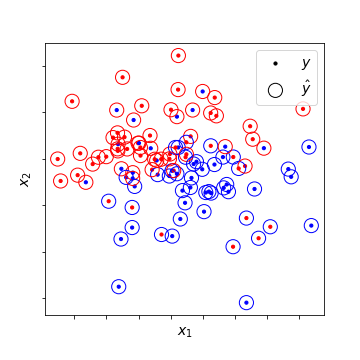
\includegraphics[width=0.85\textwidth]{../plots_teoria/intro_scatterplot.png}
								\caption{Clasificación}
							\end{minipage}
							\begin{minipage}{0.375\textwidth}
								\centering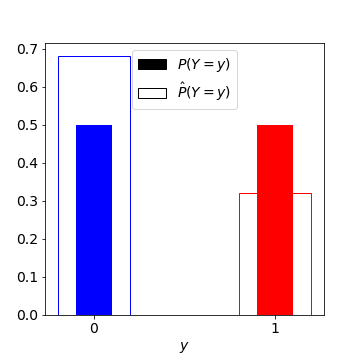
\includegraphics[width=1\textwidth]{../plots_teoria/intro_barplot.png}
								\caption{Cuantificación}
							\end{minipage}
						\end{figure}
						Sin embargo, esta estrategia (método {\it baseline} de cuantificación, conocido como
						{\it Classify \& Count -CC-\/ }) es subóptima: si bien un clasificador perfecto es
						también un cuantificador perfecto, \textbf{un buen clasificador puede ser un mal cuantificador},
						principalmente si la distribución de los datos utilizados para entrenar es diferente
						a la de los datos que se usan para predecir.
					\end{myblock}\vfill

					\begin{myblock}{Marco teórico}
						Teniendo en cuenta que en los problemas de clasificación tenemos:
						\begin{itemize}
							\item Un conjunto de características o covariables $\boldsymbol{X}$.
							\item Una variable de respuesta $Y$.
							\item Una distribución de probabilidad conjunta
							$\mathbb{P}(Y=y,\boldsymbol{X=x})$.
						\end{itemize}
						La probabilidad conjunta $\mathbb{P}(Y,\boldsymbol{X})$ se puede escribir
						como $\mathbb{P}(Y|\boldsymbol{X})\mathbb{P}(\boldsymbol{X})$ o como
						$\mathbb{P}(\boldsymbol{X}|Y)\mathbb{P}(Y)$.
						El {\it dataset shift\/} aparece cuando las distribuciones conjuntas de
						entrenamiento y de prueba son diferentes, es decir, cuando
						$\mathbb{P}_{tr}(Y,\boldsymbol{X}) \neq
						\mathbb{P}_{tst}(Y,\boldsymbol{X})$. En el caso particular de $\mathbb{P}_{tr}(\boldsymbol{X}|Y) = \mathbb{P}_{tst}(\boldsymbol{X}|Y)$ y
						$\mathbb{P}_{tr}(Y) \neq \mathbb{P}_{tst}(Y)$, se habla de {\it prior probability shift}.
						El problema de cuantificación se trata de un caso donde
						$\mathbb{P}_{tst}(Y)$ es desconocido. Además, la mayoría de los métodos de
						cuantificación propuestos asumen que $\mathbb{P}_{tr}(\boldsymbol{X}|Y) =
						\mathbb{P}_{tst}(\boldsymbol{X}|Y)$, por lo que están dentro de los casos de
						{\it prior probability shift}.
						\begin{figure}
							\begin{minipage}{0.45\textwidth}
								\centering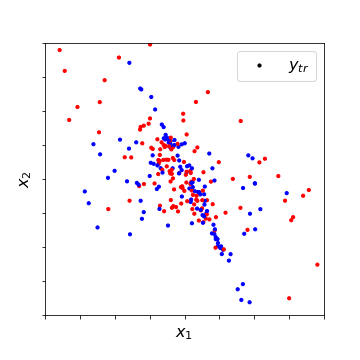
\includegraphics[width=0.85\textwidth]{../plots_teoria/cambios_train_scatterplot.png}
								\caption{Muestra de entrenamiento}
							\end{minipage}
							\hfill
							\begin{minipage}{0.45\textwidth}
								\centering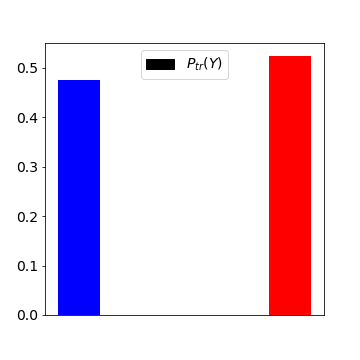
\includegraphics[width=0.85\textwidth]{../plots_teoria/cambios_train_barplot.png}
								\caption{Prevalencia de clases en muestra de entrenamiento}
							\end{minipage}
							\medskip
							\begin{minipage}{0.45\textwidth}
								\centering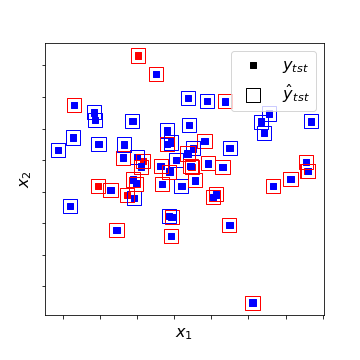
\includegraphics[width=0.85\textwidth]{../plots_teoria/cambios_test_scatterplot.png}
								\caption{Clasificación en muestra de prueba. Para el modelo, las
								$y_{tst}$ son desconocidas.}
							\end{minipage}
							\hfill
							\begin{minipage}{0.45\textwidth}
								\centering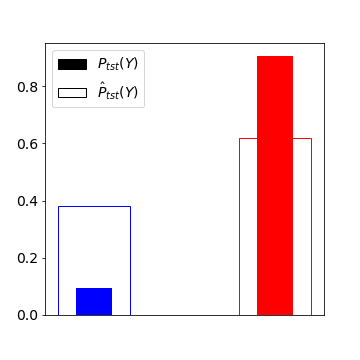
\includegraphics[width=0.85\textwidth]{../plots_teoria/cambios_test_barplot.png}
								\caption{Prevalencia de clases verdadera y cuantificación en muestra de
								prueba}
							\end{minipage}
						\end{figure}
					\end{myblock}\vfill

		}\end{minipage}\end{beamercolorbox}
	\end{column}

	\begin{column}{.57\textwidth}
		\begin{beamercolorbox}[center]{postercolumn}
			\begin{minipage}{.98\textwidth} % tweaks the width, makes a new \textwidth
				\parbox[t][\columnheight]{\textwidth}{ % must be some better way to set the the height, width and textwidth simultaneously

					\begin{myblock}{El problema de clasificar y contar}
						Bajo el supuesto de {\it prior probability shift\/}, la estimación $\hat p$
						obtenida por el enfoque {\it CC\/} depende sólo de las características
						del clasificador, definido (para el caso binario) por su tasa de verdaderos
						positivos ($tpr$), su tasa de falsos positivos ($fpr$) y de la prevalencia real
						($p$):
						\begin{equation}\label{ecuacion:tpr_fpr}
							\hat p(p) = p \cdot {tpr} + (1-p) \cdot {fpr}
						\end{equation}
						\begin{figure}[h]
							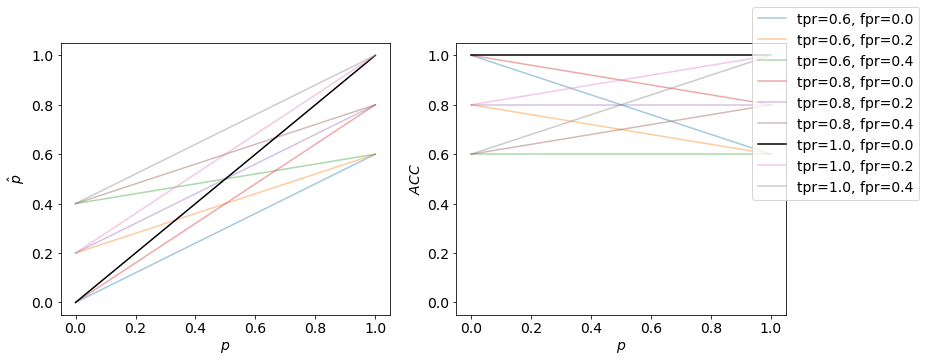
\includegraphics[width=\textwidth]{../plots_teoria/cc_tpr_fpr.png}
							\caption{La línea negra representa el cuantificador y clasificador perfecto,
							respectivamente. Las otras líneas muestran las estimaciones teóricas de
							$\hat p$ resultantes de aplicar la ecuación~\ref{ecuacion:tpr_fpr}, y el
							${\it accuracy\/}$ correspondiente al clasificador, según se varían los
							valores de $tpr$ y $fpr$}
						\end{figure}
					\end{myblock}\vfill

					\begin{myblock}{Mejora de la clasificación}
						Los métodos de cuantifacación también se pueden emplear para suplir los defectos
						de clasificadores frente a cambios en las distribuciones de los datos.
						Por ejemplo, en el caso del clasificador óptimo de Bayes, dado por:
						\begin{equation}\label{ecuacion:bayes}
							h(\boldsymbol{x}) = \argmax_{y} p_{Y|\boldsymbol{X}=\boldsymbol{x}}(y) = \argmax_{y} \frac{p_{\boldsymbol{X}|Y=y}(\boldsymbol{x})p_Y(y)}{p_{\boldsymbol{X}}(\boldsymbol{x})}
						\end{equation}
						la decisión depende de $p_Y(y)$, que suele ser estimado con los datos
						de entrenamiento. Para mejorar el rendimiento del
						clasificador, se debería usar $\hat p_Y(y) = p_{tst}$,
						pero como $p_{tst}$ suele ser desconocido, se puede usar un método de
						cuantificación para estimarlo.
					\end{myblock}\vfill

					\begin{myblock}{Métodos}
						Algunos de los principales métodos de cuantificación son:
						\begin{itemize}
							\item \textbf{Clasificar y Contar (CC):} El {\it baseline\/} ya mencionado, cuyo estimador es: 
							\begin{equation}
								\hat p^{\it{CC}}_{tst}(c=1) = \frac{\#\{\boldsymbol{x} \in \boldsymbol{X}_{tst}|h_{tr}(\boldsymbol{x})=1\}}{\#\boldsymbol{X}_{tst}}
							\end{equation}
							\item \textbf{Clasificar, Contar y Ajustar (ACC):} Corrige las estimaciones de \textbf{CC} mediante las estimaciones de
							$tpr$ y $fpr$:
							\begin{equation}
								\hat p^{\it{ACC}}_{tst}(c=1) = \frac{\hat p^{\it{CC}}_{tst}(c=1)-\hat {fpr}}{\hat {tpr}-\hat {fpr}}
							\end{equation}
							\item \textbf{Clasificar y Contar Probabilístico (PCC):} Utiliza los {\it scores\/} del clasificador, en vez de las clases predichas:
							\begin{equation}
								\hat p^{\it{PCC}}_{tst}(c=1) = \frac{1}{m} \sum \limits_{i=1}^{m}{s(\boldsymbol{x}_i, y=1)}
							\end{equation}
							\item \textbf{Clasificar, Contar y Ajustar Probabilístico (PACC):} Combina las ideas de \textbf{ACC} y \textbf{PCC}:
							\begin{equation}
								\hat p^{\it{PACC}}_{tst}(c=1) = \frac{\hat p^{\it{PCC}}_{tst}(c=1)-\hat {fp_{pa}}}{\hat {tp_{pa}} - \hat {fp_{pa}}}
							\end{equation}
							siendo $tp_{pa}$ el promedio de los {\it scores\/} para individuos de clase positiva, y $fp_{pa}$ para los de clase negativa.
							\item \textbf{Selección de Umbrales:} Busca un umbral que reduzca la
							varianza en las estimaciones de $tpr$ y $fpr$:
							\begin{itemize}
								\item MAX:\@ selecciona el umbral que maximiza $tpr-fpr$.
								\item X:\@ busca obtener $fpr=1-tpr$.
								\item T50:\@ elige el umbral con $tpr=0.5$, asumiendo que los positivos
								conforman la clase minoritaria.
								\item Median Sweep (MS):\@ para todos los umbrales que modifiquen los posibles valores de
								$fpr$ y $tpr$, obtiene las prevalencias y calcula su mediana.
							\end{itemize}
						\end{itemize}
					\end{myblock}\vfill

					\begin{myblock}{Objetivo y trabajo futuro}
						El objetivo de este trabajo es resumir el estado del arte en el área y
						evaluar mediante simulaciones los principales modelos propuestos. Como trabajo futuro,
						se sugiere proponer nuevos métodos de cuantificación, tanto para estimación puntual
						como por intervalos.
					\end{myblock}\vfill

		}\end{minipage}\end{beamercolorbox}
	\end{column}
\end{columns}
\end{frame}
\end{document}
